\hypertarget{group__STM32F3__DISCOVERY__LINK__OPERATIONS}{}\section{Link Operation functions}
\label{group__STM32F3__DISCOVERY__LINK__OPERATIONS}\index{Link Operation functions@{Link Operation functions}}
Collaboration diagram for Link Operation functions\+:\nopagebreak
\begin{figure}[H]
\begin{center}
\leavevmode
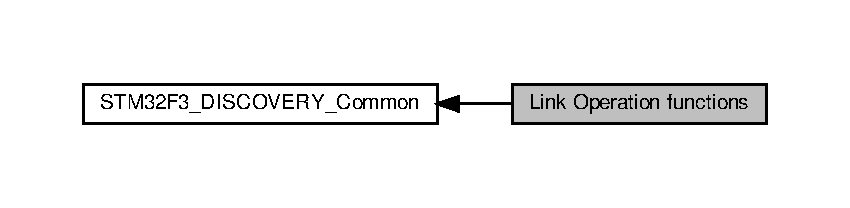
\includegraphics[width=350pt]{group__STM32F3__DISCOVERY__LINK__OPERATIONS}
\end{center}
\end{figure}


\subsection{Detailed Description}


\subsection{Function Documentation}
\mbox{\Hypertarget{group__STM32F3__DISCOVERY__LINK__OPERATIONS_ga7ce9cc034e3d64924bd88adae6770d19}\label{group__STM32F3__DISCOVERY__LINK__OPERATIONS_ga7ce9cc034e3d64924bd88adae6770d19}} 
\index{Link Operation functions@{Link Operation functions}!C\+O\+M\+P\+A\+S\+S\+A\+C\+C\+E\+L\+E\+R\+O\+\_\+\+I\+O\+\_\+\+Init@{C\+O\+M\+P\+A\+S\+S\+A\+C\+C\+E\+L\+E\+R\+O\+\_\+\+I\+O\+\_\+\+Init}}
\index{C\+O\+M\+P\+A\+S\+S\+A\+C\+C\+E\+L\+E\+R\+O\+\_\+\+I\+O\+\_\+\+Init@{C\+O\+M\+P\+A\+S\+S\+A\+C\+C\+E\+L\+E\+R\+O\+\_\+\+I\+O\+\_\+\+Init}!Link Operation functions@{Link Operation functions}}
\subsubsection{\texorpdfstring{C\+O\+M\+P\+A\+S\+S\+A\+C\+C\+E\+L\+E\+R\+O\+\_\+\+I\+O\+\_\+\+Init()}{COMPASSACCELERO\_IO\_Init()}}
{\footnotesize\ttfamily void C\+O\+M\+P\+A\+S\+S\+A\+C\+C\+E\+L\+E\+R\+O\+\_\+\+I\+O\+\_\+\+Init (\begin{DoxyParamCaption}\item[{void}]{ }\end{DoxyParamCaption})}



Configures C\+O\+M\+P\+A\+SS / A\+C\+C\+E\+L\+E\+R\+O\+M\+E\+T\+ER I2C interface. 


\begin{DoxyRetVals}{Return values}
{\em None} & \\
\hline
\end{DoxyRetVals}
\mbox{\Hypertarget{group__STM32F3__DISCOVERY__LINK__OPERATIONS_ga0d94d79fddfe98ed16c8c63c65f186db}\label{group__STM32F3__DISCOVERY__LINK__OPERATIONS_ga0d94d79fddfe98ed16c8c63c65f186db}} 
\index{Link Operation functions@{Link Operation functions}!C\+O\+M\+P\+A\+S\+S\+A\+C\+C\+E\+L\+E\+R\+O\+\_\+\+I\+O\+\_\+\+I\+T\+Config@{C\+O\+M\+P\+A\+S\+S\+A\+C\+C\+E\+L\+E\+R\+O\+\_\+\+I\+O\+\_\+\+I\+T\+Config}}
\index{C\+O\+M\+P\+A\+S\+S\+A\+C\+C\+E\+L\+E\+R\+O\+\_\+\+I\+O\+\_\+\+I\+T\+Config@{C\+O\+M\+P\+A\+S\+S\+A\+C\+C\+E\+L\+E\+R\+O\+\_\+\+I\+O\+\_\+\+I\+T\+Config}!Link Operation functions@{Link Operation functions}}
\subsubsection{\texorpdfstring{C\+O\+M\+P\+A\+S\+S\+A\+C\+C\+E\+L\+E\+R\+O\+\_\+\+I\+O\+\_\+\+I\+T\+Config()}{COMPASSACCELERO\_IO\_ITConfig()}}
{\footnotesize\ttfamily void C\+O\+M\+P\+A\+S\+S\+A\+C\+C\+E\+L\+E\+R\+O\+\_\+\+I\+O\+\_\+\+I\+T\+Config (\begin{DoxyParamCaption}\item[{void}]{ }\end{DoxyParamCaption})}



Configures C\+O\+M\+P\+A\+SS / A\+C\+C\+E\+L\+E\+RO click IT. 


\begin{DoxyRetVals}{Return values}
{\em None} & \\
\hline
\end{DoxyRetVals}
\mbox{\Hypertarget{group__STM32F3__DISCOVERY__LINK__OPERATIONS_ga2d4c2b7ccef8b3be4cf0335e9fcffd2f}\label{group__STM32F3__DISCOVERY__LINK__OPERATIONS_ga2d4c2b7ccef8b3be4cf0335e9fcffd2f}} 
\index{Link Operation functions@{Link Operation functions}!C\+O\+M\+P\+A\+S\+S\+A\+C\+C\+E\+L\+E\+R\+O\+\_\+\+I\+O\+\_\+\+Read@{C\+O\+M\+P\+A\+S\+S\+A\+C\+C\+E\+L\+E\+R\+O\+\_\+\+I\+O\+\_\+\+Read}}
\index{C\+O\+M\+P\+A\+S\+S\+A\+C\+C\+E\+L\+E\+R\+O\+\_\+\+I\+O\+\_\+\+Read@{C\+O\+M\+P\+A\+S\+S\+A\+C\+C\+E\+L\+E\+R\+O\+\_\+\+I\+O\+\_\+\+Read}!Link Operation functions@{Link Operation functions}}
\subsubsection{\texorpdfstring{C\+O\+M\+P\+A\+S\+S\+A\+C\+C\+E\+L\+E\+R\+O\+\_\+\+I\+O\+\_\+\+Read()}{COMPASSACCELERO\_IO\_Read()}}
{\footnotesize\ttfamily uint8\+\_\+t C\+O\+M\+P\+A\+S\+S\+A\+C\+C\+E\+L\+E\+R\+O\+\_\+\+I\+O\+\_\+\+Read (\begin{DoxyParamCaption}\item[{uint16\+\_\+t}]{Device\+Addr,  }\item[{uint8\+\_\+t}]{Register\+Addr }\end{DoxyParamCaption})}



Reads a block of data from the C\+O\+M\+P\+A\+SS / A\+C\+C\+E\+L\+E\+R\+O\+M\+E\+T\+ER. 


\begin{DoxyParams}{Parameters}
{\em Device\+Addr} & specifies the slave address to be programmed(\+A\+C\+C\+\_\+\+I2\+C\+\_\+\+A\+D\+D\+R\+E\+S\+S or M\+A\+G\+\_\+\+I2\+C\+\_\+\+A\+D\+D\+R\+E\+S\+S). \\
\hline
{\em Register\+Addr} & specifies the C\+O\+M\+P\+A\+SS / A\+C\+C\+E\+L\+E\+R\+O\+M\+E\+T\+ER internal address register to read from \\
\hline
\end{DoxyParams}

\begin{DoxyRetVals}{Return values}
{\em A\+C\+C\+E\+L\+E\+R\+O\+M\+E\+T\+ER} & register value \\
\hline
\end{DoxyRetVals}
\mbox{\Hypertarget{group__STM32F3__DISCOVERY__LINK__OPERATIONS_gad84492b8ff84b8112e4e93d35d67f116}\label{group__STM32F3__DISCOVERY__LINK__OPERATIONS_gad84492b8ff84b8112e4e93d35d67f116}} 
\index{Link Operation functions@{Link Operation functions}!C\+O\+M\+P\+A\+S\+S\+A\+C\+C\+E\+L\+E\+R\+O\+\_\+\+I\+O\+\_\+\+Write@{C\+O\+M\+P\+A\+S\+S\+A\+C\+C\+E\+L\+E\+R\+O\+\_\+\+I\+O\+\_\+\+Write}}
\index{C\+O\+M\+P\+A\+S\+S\+A\+C\+C\+E\+L\+E\+R\+O\+\_\+\+I\+O\+\_\+\+Write@{C\+O\+M\+P\+A\+S\+S\+A\+C\+C\+E\+L\+E\+R\+O\+\_\+\+I\+O\+\_\+\+Write}!Link Operation functions@{Link Operation functions}}
\subsubsection{\texorpdfstring{C\+O\+M\+P\+A\+S\+S\+A\+C\+C\+E\+L\+E\+R\+O\+\_\+\+I\+O\+\_\+\+Write()}{COMPASSACCELERO\_IO\_Write()}}
{\footnotesize\ttfamily void C\+O\+M\+P\+A\+S\+S\+A\+C\+C\+E\+L\+E\+R\+O\+\_\+\+I\+O\+\_\+\+Write (\begin{DoxyParamCaption}\item[{uint16\+\_\+t}]{Device\+Addr,  }\item[{uint8\+\_\+t}]{Register\+Addr,  }\item[{uint8\+\_\+t}]{Value }\end{DoxyParamCaption})}



Writes one byte to the C\+O\+M\+P\+A\+SS / A\+C\+C\+E\+L\+E\+R\+O\+M\+E\+T\+ER. 


\begin{DoxyParams}{Parameters}
{\em Device\+Addr} & specifies the slave address to be programmed. \\
\hline
{\em Register\+Addr} & specifies the C\+O\+M\+P\+A\+SS / A\+C\+C\+E\+L\+E\+R\+O\+M\+E\+T\+ER register to be written. \\
\hline
{\em Value} & Data to be written \\
\hline
\end{DoxyParams}

\begin{DoxyRetVals}{Return values}
{\em None} & \\
\hline
\end{DoxyRetVals}
\mbox{\Hypertarget{group__STM32F3__DISCOVERY__LINK__OPERATIONS_gab11396b3a6f76ba95ea19290c7e60da5}\label{group__STM32F3__DISCOVERY__LINK__OPERATIONS_gab11396b3a6f76ba95ea19290c7e60da5}} 
\index{Link Operation functions@{Link Operation functions}!G\+Y\+R\+O\+\_\+\+I\+O\+\_\+\+Init@{G\+Y\+R\+O\+\_\+\+I\+O\+\_\+\+Init}}
\index{G\+Y\+R\+O\+\_\+\+I\+O\+\_\+\+Init@{G\+Y\+R\+O\+\_\+\+I\+O\+\_\+\+Init}!Link Operation functions@{Link Operation functions}}
\subsubsection{\texorpdfstring{G\+Y\+R\+O\+\_\+\+I\+O\+\_\+\+Init()}{GYRO\_IO\_Init()}}
{\footnotesize\ttfamily void G\+Y\+R\+O\+\_\+\+I\+O\+\_\+\+Init (\begin{DoxyParamCaption}\item[{void}]{ }\end{DoxyParamCaption})}



Configures the G\+Y\+R\+O\+S\+C\+O\+PE S\+PI interface. 


\begin{DoxyRetVals}{Return values}
{\em None} & \\
\hline
\end{DoxyRetVals}
\mbox{\Hypertarget{group__STM32F3__DISCOVERY__LINK__OPERATIONS_ga1432dd354981626497d038b4f7149b92}\label{group__STM32F3__DISCOVERY__LINK__OPERATIONS_ga1432dd354981626497d038b4f7149b92}} 
\index{Link Operation functions@{Link Operation functions}!G\+Y\+R\+O\+\_\+\+I\+O\+\_\+\+Read@{G\+Y\+R\+O\+\_\+\+I\+O\+\_\+\+Read}}
\index{G\+Y\+R\+O\+\_\+\+I\+O\+\_\+\+Read@{G\+Y\+R\+O\+\_\+\+I\+O\+\_\+\+Read}!Link Operation functions@{Link Operation functions}}
\subsubsection{\texorpdfstring{G\+Y\+R\+O\+\_\+\+I\+O\+\_\+\+Read()}{GYRO\_IO\_Read()}}
{\footnotesize\ttfamily void G\+Y\+R\+O\+\_\+\+I\+O\+\_\+\+Read (\begin{DoxyParamCaption}\item[{uint8\+\_\+t$\ast$}]{p\+Buffer,  }\item[{uint8\+\_\+t}]{Read\+Addr,  }\item[{uint16\+\_\+t}]{Num\+Byte\+To\+Read }\end{DoxyParamCaption})}



Reads a block of data from the G\+Y\+R\+O\+S\+C\+O\+PE. 


\begin{DoxyParams}{Parameters}
{\em p\+Buffer} & pointer to the buffer that receives the data read from the G\+Y\+R\+O\+S\+C\+O\+PE. \\
\hline
{\em Read\+Addr} & G\+Y\+R\+O\+S\+C\+O\+PE\textquotesingle{}s internal address to read from. \\
\hline
{\em Num\+Byte\+To\+Read} & number of bytes to read from the G\+Y\+R\+O\+S\+C\+O\+PE. \\
\hline
\end{DoxyParams}

\begin{DoxyRetVals}{Return values}
{\em None} & \\
\hline
\end{DoxyRetVals}
\mbox{\Hypertarget{group__STM32F3__DISCOVERY__LINK__OPERATIONS_ga5d9e3e80db2ee7cb6d8bd2f92d25b339}\label{group__STM32F3__DISCOVERY__LINK__OPERATIONS_ga5d9e3e80db2ee7cb6d8bd2f92d25b339}} 
\index{Link Operation functions@{Link Operation functions}!G\+Y\+R\+O\+\_\+\+I\+O\+\_\+\+Write@{G\+Y\+R\+O\+\_\+\+I\+O\+\_\+\+Write}}
\index{G\+Y\+R\+O\+\_\+\+I\+O\+\_\+\+Write@{G\+Y\+R\+O\+\_\+\+I\+O\+\_\+\+Write}!Link Operation functions@{Link Operation functions}}
\subsubsection{\texorpdfstring{G\+Y\+R\+O\+\_\+\+I\+O\+\_\+\+Write()}{GYRO\_IO\_Write()}}
{\footnotesize\ttfamily void G\+Y\+R\+O\+\_\+\+I\+O\+\_\+\+Write (\begin{DoxyParamCaption}\item[{uint8\+\_\+t$\ast$}]{p\+Buffer,  }\item[{uint8\+\_\+t}]{Write\+Addr,  }\item[{uint16\+\_\+t}]{Num\+Byte\+To\+Write }\end{DoxyParamCaption})}



Writes one byte to the G\+Y\+R\+O\+S\+C\+O\+PE. 


\begin{DoxyParams}{Parameters}
{\em p\+Buffer} & pointer to the buffer containing the data to be written to the G\+Y\+R\+O\+S\+C\+O\+PE. \\
\hline
{\em Write\+Addr} & G\+Y\+R\+O\+S\+C\+O\+PE\textquotesingle{}s internal address to write to. \\
\hline
{\em Num\+Byte\+To\+Write} & Number of bytes to write. \\
\hline
\end{DoxyParams}

\begin{DoxyRetVals}{Return values}
{\em None} & \\
\hline
\end{DoxyRetVals}
